% !TEX root = ../report.tex

\section{Logical View}
\label{sec:viewlogical}

% Logical view : The logical view is concerned with the functionality that the system provides to end-users. UML Diagrams used to represent the logical view include Class diagram, Communication diagram, Sequence diagram.

\begin{figure}[H]
\caption{An high-level overview of the Docker architecture. Source: \cite{dockerarchi}.}
\centering
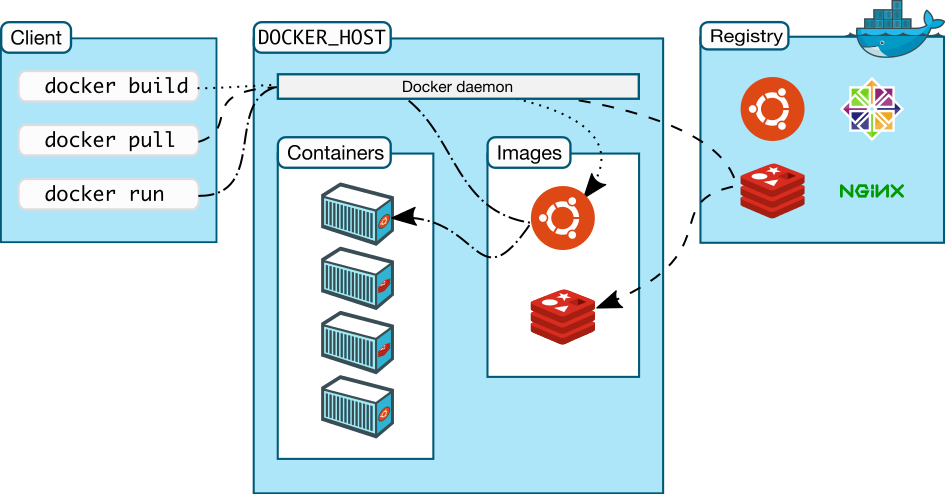
\includegraphics[scale=0.4]{4-softwarearch/images/architecture.png}
\label{fig:dockerarchipic}
\end{figure}
Docker uses a client-server architecture. The client (a command-line tool) acts as the primary user interface and talks to the Docker daemon. The daemon is a background process which does all the heavy lifting, e.g. the building and running of the containers.

\subsection{Client}
The client is a small binary and acts as the primary user interface to Docker. The user enters command into the client and the client forwards these commands to the Docker daemon, which executes commands.
The Docker client is capable of connecting to daemons running on the local machine, as well as connecting to daemons running on remote machines over the internet.

\subsection{Server / Daemon}
The Docker daemon is a process running on the host machine (as can be seen in Figure~\ref{fig:dockerarchipic}). This process is started when the host machine starts and runs in the background. It exposes a REST interface and listens for requests coming from clients on the same or remote hosts.

%As shown in the diagram above, the Docker daemon runs on a host machine. The user does not directly interact with the daemon, but instead through the Docker client.

\subsubsection{Images}
Docker images can be interpreted as a template from which Docker containers are
started. A Docker image consists of a stack of layers which are bonded by union
file systems. These layers support reusability and sharing.

\subsubsection{Containers}
Docker containers are based on Docker images. This image acts as a read-only
layers. Then, Docker container adds up a thin writable layer on top of it to
perform operations. Docker containers basically consists of an operating system,
user-added files, application, and some information. Multiple containers may run
based on a same image. In this case, Docker will not create separate copies for
each containers. Instead, they will share same image with their own writable
thin layer.

\subsection{Registry}
The Docker registry is the place where Docker images are stored. Docker daemon
fetches desired Docker images from this repository. This registry may be a
public or a private one, such as one behind firewall. Docker
Hub\footnote{\url{https://hub.docker.com/}} is one example of a docker registry
hosted by Docker. This registry provides
